\chapter{Result and Discussion} \label{chp:result}

The performance of GBM will be evaluated by means of a case study using the test dataset. The test dataset comprises journey data from the month of June. The first part will focus on performance evaluation of BBM, where the trained model will be used to predict the SOG. The second part focus on the power estimation method using Holtrop-Mennen method. The output of BBM, which is the ship SOG, will be fed to the WBM to estimate the power. The generated power speed curve models the journey in the month of June which considered the weather effects and the dynamics of the ship.

\section{Evaluation of Tree-based model}\label{sec:BBM_tree_evaluate}

\subsection*{Model Training and Selection of Optimal Parameter}\label{sec:hpo_select_train}

Putting aside the test dataset, the training and validation dataset is split to 80:20 ratio which correspond to 2804 training data and 702 validation data. The initial training uses default hyperparameter and the performance of the model is evaluated using the validation dataset using k-cross validation. To help narrow the search range of each hyperparameter, RMSE plots against different values of hyperparameters will be performed. This method was presented in \Cref{sec:hpo}. The hyperparameter will be iteratively tuned until the best model is obtained. The result of the optimal parameter is found in \Cref{tbl:hpo_optimal}. The model training is executed using \textbf{AMD Ryzen 7 2700X, Eight-Core Processor $@$ 3.7 GHz processor with 16384 MB installed RAM}.\\


\begin{table}[ht]
    \footnotesize
    \centering
    % \resizebox {\textwidth}{!}
    {\begin{tabular}{ p{0.1\linewidth} p{0.2\linewidth} p{0.3\linewidth}}
    \hline
    Model & Training time [s] & Optimal Hyperparameter \\
    \hline
    DTR & 0.044 & None \\
    $\text{DTR}_{OPT}$ & 0.021  & {\tt min\_samples\_split = 7}\\
    &&{\tt min\_samples\_leaf = 10}\\
    &&{\tt max\_features = 12}\\
    &&{\tt max\_depth = 8}\\
    RFR & 4.112 & None \\
    $\text{RFR}_{OPT}$ & 3.431  & {\tt min\_samples\_split = 2}\\
    &&{\tt min\_samples\_leaf = 1}\\
    &&{\tt max\_features = 10}\\
    &&{\tt max\_depth = 120}\\
    &&{\tt n\_estimators = 100}\\
    ETR & 0.944 & None \\
    $\text{ETR}_{OPT}$ & 4.390  & {\tt min\_samples\_split = 9}\\
    &&{\tt min\_samples\_leaf = 1}\\
    &&{\tt max\_features = 12}\\
    &&{\tt max\_depth = 120}\\
    &&{\tt n\_estimators = 800}\\
    MLR & 0.004  & None\\
    \hline
    \end{tabular}}
\caption{Optimal hyperparameter with training time of each model}\label{tbl:hpo_optimal}
\end{table}

With the default hyperparameter, RFR takes the longest training time followed by ETR and DTR. This is expected as RFR uses greedy algorithm i.e. it looks for the best possible feature when splitting the node. ETR takes significantly shorter time to train as ETR randomly select for features when splitting the node. DTR takes the shortest training time as it only generates a single tree.\\

However, in the case of optimised model, ETR takes a longer time to train compared to RFR. This is caused by the number of trees in the optimised model which is controlled by the parameter {\tt n\_estimator}, the optimised ETR model has 800 trees in comparison to 100 trees of RFR. It is also observed that the training time of optimised DTR model is halved as pruning the tree resulted in a simpler model to train. \\

To further investigate the effect of hyperparameter optimisation, the learning curve of each tree-based model is plotted. For DTR, generated model with default parameter will result in a model that heavily overfits the training data, evident from the high variance shown in \Cref{fig:learn_curve_DTR_RMSE}. Regularisation of the DTR model helps balance between bias and variance, this balancing process trades bias for variance, as observed from the substantial reduction in the gap between the training and validation error. Additionally, the learning curve indicates that the most notable improvement in model performance occurs until around 1200 data points. Beyond this point, the enhancement in model performance becomes less substantial.\\

\begin{figure}[h]
    \centering
        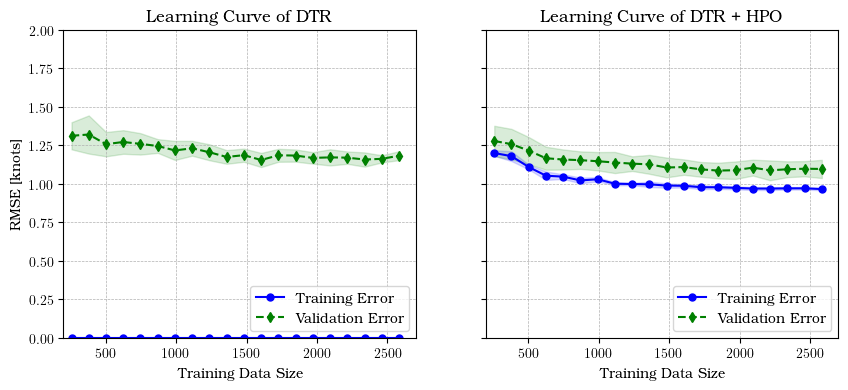
\includegraphics[width=.95\textwidth]{02_figures/learning_curve_dtr.png}
        \caption{Learning curve of DTR}
        \label{fig:learn_curve_DTR_RMSE}
\end{figure}

The process of hyperparameter tuning for the Random Forest Regressor (RFR) model did not show any significant improvement in model performance. This outcome aligns with the findings of  \bcitet{Kuhn.2013} and \bcitet{Hastie.2009} which was discussed in \Cref{sec:rf_theo}. The most notable improvement on model performance is observed until around 750 points, after which the model appears to reach a plateau. Furthermore, there is noticeable variance in the RFR model, which indicates that the model will have a slight tendency to overfit.

\begin{figure}[h]
    \centering
        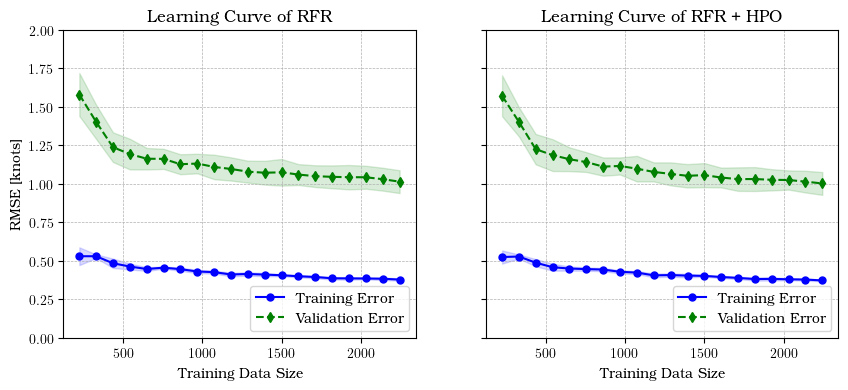
\includegraphics[width=.95\textwidth]{02_figures/learning_curve_rfr_rmse.png}
        \caption{Learning curve of RFR}
        \label{fig:learn_curve_RFR_RMSE}
\end{figure}

Hyperparameter tuning helps to reduce variance in the ETR model. Similar to the Random Forest Regressor (RFR), a significant increase in model performance is achieved until approximately 750 data points. However, beyond this point, both the RFR and ETR models reach a plateau, indicating that adding more data points will not further improve the model performance.

\begin{figure}[h]
    \centering
        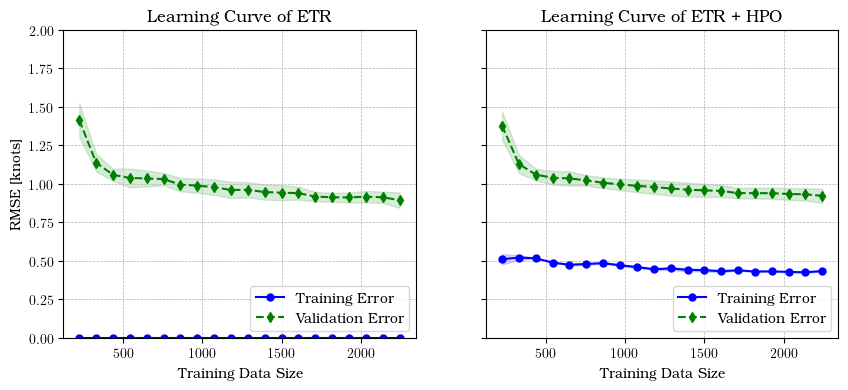
\includegraphics[width=.95\textwidth]{02_figures/learning_curve_etr_rmse.png}
        \caption{Learning curve of ETR}
        \label{fig:learn_curve_ETR_RMSE}
\end{figure}


\subsection*{Evaluation of trained model}\label{sec:BBM_model_eval}

To ensure accu

